\documentclass{article}\usepackage[]{graphicx}\usepackage[]{color}
% maxwidth is the original width if it is less than linewidth
% otherwise use linewidth (to make sure the graphics do not exceed the margin)
\makeatletter
\def\maxwidth{ %
  \ifdim\Gin@nat@width>\linewidth
    \linewidth
  \else
    \Gin@nat@width
  \fi
}
\makeatother

\definecolor{fgcolor}{rgb}{0.345, 0.345, 0.345}
\newcommand{\hlnum}[1]{\textcolor[rgb]{0.686,0.059,0.569}{#1}}%
\newcommand{\hlstr}[1]{\textcolor[rgb]{0.192,0.494,0.8}{#1}}%
\newcommand{\hlcom}[1]{\textcolor[rgb]{0.678,0.584,0.686}{\textit{#1}}}%
\newcommand{\hlopt}[1]{\textcolor[rgb]{0,0,0}{#1}}%
\newcommand{\hlstd}[1]{\textcolor[rgb]{0.345,0.345,0.345}{#1}}%
\newcommand{\hlkwa}[1]{\textcolor[rgb]{0.161,0.373,0.58}{\textbf{#1}}}%
\newcommand{\hlkwb}[1]{\textcolor[rgb]{0.69,0.353,0.396}{#1}}%
\newcommand{\hlkwc}[1]{\textcolor[rgb]{0.333,0.667,0.333}{#1}}%
\newcommand{\hlkwd}[1]{\textcolor[rgb]{0.737,0.353,0.396}{\textbf{#1}}}%
\let\hlipl\hlkwb

\usepackage{framed}
\makeatletter
\newenvironment{kframe}{%
 \def\at@end@of@kframe{}%
 \ifinner\ifhmode%
  \def\at@end@of@kframe{\end{minipage}}%
  \begin{minipage}{\columnwidth}%
 \fi\fi%
 \def\FrameCommand##1{\hskip\@totalleftmargin \hskip-\fboxsep
 \colorbox{shadecolor}{##1}\hskip-\fboxsep
     % There is no \\@totalrightmargin, so:
     \hskip-\linewidth \hskip-\@totalleftmargin \hskip\columnwidth}%
 \MakeFramed {\advance\hsize-\width
   \@totalleftmargin\z@ \linewidth\hsize
   \@setminipage}}%
 {\par\unskip\endMakeFramed%
 \at@end@of@kframe}
\makeatother

\definecolor{shadecolor}{rgb}{.97, .97, .97}
\definecolor{messagecolor}{rgb}{0, 0, 0}
\definecolor{warningcolor}{rgb}{1, 0, 1}
\definecolor{errorcolor}{rgb}{1, 0, 0}
\newenvironment{knitrout}{}{} % an empty environment to be redefined in TeX

\usepackage{alltt}
\usepackage{Sweave}
\usepackage{float}
\usepackage{subcaption}
\usepackage{graphicx}
\usepackage{tabularx}
\usepackage{siunitx}
\usepackage{multirow}
\usepackage{amssymb} % for math symbols
\usepackage{amsmath} % for aligning equations
%\usepackage{hyperref}
\usepackage{textcomp}
\usepackage{mdframed}
\usepackage{natbib}
\bibliographystyle{..//bib/styles/gcb}
%\usepackage[hyphens]{url}
\usepackage{caption}
\setlength{\captionmargin}{30pt}
\setlength{\abovecaptionskip}{0pt}
\setlength{\belowcaptionskip}{10pt}
\topmargin -1.5cm        
\oddsidemargin -0.04cm   
\evensidemargin -0.04cm
\textwidth 16.59cm
\textheight 21.94cm 
%\pagestyle{empty} %comment if want page numbers
\parskip 7.2pt
\renewcommand{\baselinestretch}{1.5}
\parindent 0pt
\usepackage{lineno}
\linenumbers

\newmdenv[
  topline=true,
  bottomline=true,
  skipabove=\topsep,
  skipbelow=\topsep
]{siderules}

%% R Script


\IfFileExists{upquote.sty}{\usepackage{upquote}}{}
\begin{document}
\noindent \textbf{\Large{Supplemental materials:}}\\
{\textbf{\Large{Climate change increases the risk of false springs in European trees}} \\
OR \\
\textbf{\Large{False spring risk increases across European trees in the face of climate change}} \\
OR \\
\textbf{\Large{Heightened risk of false springs with climate change across six European tree species}}


\noindent Authors:\\
C. J. Chamberlain $^{1,2}$, B. I. Cook $^{3}$, I. Morales-Castilla $^{4,5}$ \& E. M. Wolkovich $^{1,2,6}$
\vspace{2ex}\\
\emph{Author affiliations:}\\
$^{1}$Arnold Arboretum of Harvard University, 1300 Centre Street, Boston, Massachusetts, USA; \\
$^{2}$Organismic \& Evolutionary Biology, Harvard University, 26 Oxford Street, Cambridge, Massachusetts, USA; \\
$^{3}$NASA Goddard Institute for Space Studies, New York, New York, USA; \\
$^{4}$GloCEE - Global Change Ecology and Evolution Group, Department of Life Sciences, Universidad de Alcal\'{a}, Alcal\'{a} de Henares, 28805, Spain \\
$^{5}$Department of Environmental Science and Policy, George Mason University, Fairfax, VA 22030; \\
$^{6}$Forest \& Conservation Sciences, Faculty of Forestry, University of British Columbia, 2424 Main Mall, Vancouver, BC V6T 1Z4\\
\vspace{2ex}
$^*$Corresponding author: 248.953.0189; cchamberlain@g.harvard.edu\\

\renewcommand{\thetable}{\arabic{table}}
\renewcommand{\thefigure}{\arabic{figure}}
\renewcommand{\labelitemi}{$-$}
\setkeys{Gin}{width=0.8\textwidth}

\section*{Methods: Spatial predictor} %I'm not too sure about the 'space parameter' terminology, I'd rather use either spatial or geographic predictor or proxy. I'm using spatial predictor, but all our predictors are spatial, so please feel free to change.

Spatial autocorrelation (SA) is a common issue in spatial ecology given that nearby spatial units tend to be more similar than units far apart, and thus, cannot be considered as independent units, which is a frequent assumption in statistical tests \citep{diniz2003spatial}. If model residuals are spatially autocorrelated, and thus, non-independent then model coefficients and errors may be biased in a hard-to-predict way \citep{mauricio2009coefficient}. On the contrary, if model residuals are not autocorrelated, then SA should not be of concern \citep{hawkins2012eight}.\\

To control for spatial autocorrelation and to account for spatially structured processes independent from our environmental predictors of false springs, we generated an additional spatial predictor for the model. To avoid collinearity, we computed our spatial predictor from the residuals of a linear model of false springs as a function (Equation S1) of all other factors that are also spatially structured (e.g. spring temperature, altitude, distance to the coast), following the logic of spatial filter modelling \citep{diniz2005modelling}. The calculation of the spatial predictor followed the next steps: (a) we fit a linear model of false spring versus environmental factors, (b) we extracted the residuals of the regression Equation S1, which represent the portion of the variation in the number of false springs that is independent from the predictors in the model and (c) we utilized the residuals as our \textit{y\textsubscript{i}} values in a selection of spatial eigenvectors to retain only the minimal subset of spatial eigenvectors that are able to remove SA from model residuals. Specifically, we selected eigenvectors following the the minimization of Moran's \textit{I} of the residuals (MIR) approach \citep{griffith2006spatial,diniz2012selection,Baumen2017}. (d) Next, we fit a linear model between the residuals of Equation S1 and the subset of selected eigenvectors. And, finally, (e) we took the fitted values from this regression as our spatial predictor in our final model (see equation from main text, Equation 1), which can be interpreted as a latent variable summarizing the spatial structure in false springs that is unaccounted for by the rest of the environmental factors in our model \citep{morales2012imprint}. A spatial predictor generated in this way has three major advantages. First, it ensures that no SA is left in model residuals. Second, it avoids introducing collinearity issues with other predictors in the model. And third, it can be interpreted as a latent variable summarizing spatial processes (e.g. local adaptation, plasticity, etc.) occurring at multiple scales.

\begin{align*}
y_i = \alpha_{[i]} +&  \beta_{NAO_{[i]}} + \beta_{MST_{[i]}} + \beta_{Elevation_{[i]}} + \beta_{DistanceCoast_{[i]}} \\ +& \beta_{ClimateChange_{[i]}}
+ \beta_{NAO \times Species_{[i]}} + \beta_{MST \times Species_{[i]}} + \beta_{Elevation \times Species_{[i]}} \\ +& \beta_{DistanceCoast \times Species_{[i]}} + \beta_{ClimateChange \times Species_{[i]}} \\
+& \beta_{NAO \times ClimateChange_{[i]}} + \beta_{MST \times ClimateChange_{[i]}} 
+ \beta_{Elevation \times ClimateChange_{[i]}} \\ +& \beta_{DistanceCoast \times ClimateChange_{[i]}} + \sigma_{[i]} \tag{S1}
\end{align*}


\section*{Species rate of budburst calculations}
Due to the paucity of data for BBCH 7 in the PEP725 dataset, we were unable to use observations for both budburst and leafout to determine the durations of vegetative risk. Instead, we used data from a growth chamber experiment \citep{Flynn2018} to determine the average number of days between budburst and leafout for our study species. %Cuttings for the experiment were made in January 2015 from two field sites: Harvard Forest (HF, 42.5$^{\circ}$N, 72.2$^{\circ}$W) and the Station de Biologie des Laurentides in St-Hippolyte, Qu\'ebec (SH, 45.9$^{\circ}$N, 74.0$^{\circ}$W). The experiment examined budburst and leafout for \textit{Acer saccharum} (Marshall), \textit{Alnus incana} (L.), \textit{Betula papyrifera} (Marshall), \textit{Fagus grandifolia} (Ehrh.), \textit{Fraxinus nigra} (Marshall), and \textit{Quercus alba} (L.) in a fully crossed design of three levels of chilling (field chilling, field chilling plus 30 days at either 1 or 4 $^{\circ}$C), two levels of forcing (20$^{\circ}$C/10$^{\circ}$C or 15$^{\circ}$C/5$^{\circ}$C day/night temperatures, such that thermoperiodicity followed photoperiod) and two levels of photoperiod (8 versus 12 hour days) resulting in 12 treatment combinations. Phenological observations of each cutting were made every 2-3 days over 82 days. Phenology was assessed using a BBCH scale that was modified for trees \citep{Finn2007}. 
We took the mean number of days between budburst and leafout for the entire experiment, which was 12 days. We compared this number to a field observation study \citep{Donnelly2017} that looked at the time between budburst and leafout across 10 species over 5 years. Finally, we assessed data that were provided by the USA National Phenology Network and the many participants who contribute to its Nature's Notebook program (USA-NPN,2019; www.usanpn.org/data/observational) for \textit{Aesculus flava} (Sol.), \textit{Aesculus glabra} (Willd.), \textit{Alnus incana} (Moench.), \textit{Betula nigra} (L.), \textit{Betula papyrifera} (Marshall), \textit{Fagus grandifolia} (Ehrh.), \textit{Fraxinus americana} (L.), \textit{Fraxinus nigra} (Marshall) and \textit{Quercus velutina} (Lam.) and took the mean number of days between budburst and leafout. Across all three approaches, the average number of days between budburst and leafout was approximately 12 days.  

Again, due to a lack of BBCH 7 data, we were unable to determine species-specific averages of number of days between budburst and leafout. We used a similar approach as above by using data from the growth chamber experiment \citep{Flynn2018} but instead of finding whole experiment means we determined species-specific averages. We used the rate of budburst of \textit{Acer saccharum} (Marshall) for \textit{Aesculus hippocastanum} \citep{Buerki2010}, \textit{Alnus incana} for \textit{Alnus glutinosa}, \textit{Betula papyrifera} for \textit{Betula pendula} \citep{Wang2016}, \textit{Fagus grandifolia} for \textit{Fagus sylvatica}, \textit{Fraxinus nigra} for \textit{Fraxinus excelsior} and \textit{Quercus alba} (L.) for \textit{Quercus robur} \citep{Hipp2017}.

\section*{Results: The effects of climatic and spatial variation on false spring incidence}
Most species had mean spring temperatures that ranged from -5$^{\circ}$C to 12$^{\circ}$C, but for \textit{Alnus glutinosa} and \textit{Fraxinus excelsior} temperatures rarely dropped below 0$^{\circ}$C, whereas \textit{Quercus robur} experienced some of the lowest spring temperatures (see Figure S\ref{fig:mst}). 
% Given that Ben is always complainig about Figure 2, how about moving it to the supp? We have plenty of good figures. 

The overall model output estimates are for \textit{Aesculus hippocastanum} as species were used as two-way interactions to simulate modeled groups on the main effects. The model estimates on the logit scale were converted to probability percentages for easier interpretation by using the `divide by 4' rule \citep{Gelman2006} and then back converted to the original scale. %To convert we used the equations below \citep{Gelman2006}:

\iffalse
\begin{align*}
inverselogit = & (1/(1+exp(-(Model Estimate)))) \tag{S2} 
\end{align*}
\begin{align*}
inverselogit(Intercept &+ (Model Estimate/(sd(Raw Data Predictor)*2))*mean(Raw Data Predictor)) - \\ & inverselogit(Intercept + (Model Estimate/(sd(Raw Data Predictor)*2)) \\ & *(mean(Raw Data Predictor)-(2*sd(Raw Data Predictor))) * 100 \tag{S3} 
\end{align*}
\fi

\newpage
\nocite{NPN2019}
\bibliography{..//bib/regionalrisk.bib}

\newpage
\section*{Supplement: Tables and Figures}
%{\begin{figure} [H]
%  -\begin{center}
%  -\includegraphics[width=12cm]{..//figures/FS_Diff.pdf}
%  -\caption{Number of years with freezing events that occured before temperature shifts related to climate change began (1951-1983) as compared to after reported climate shifts (1984-2016). If temperatures fell below -2$^{\circ}$C between March 1 and June 30, a year with a spring freeze was tallied. Some regions experienced more years with spring freezes after climate change began, whereas other years experienced the same number or even fewer years with spring freezes. Regions that had more years with spring freezes after climate change began are blue and green and regions that had fewer freezes are depicted in red.}\label{fig:region}
%  -\end{center}
%  -\end{figure}}
  
\begin{center}
\captionof{table}{Data collected from PEP725 for each species and the calculated number of false spring years} \label{tab:spp} 
\begin{tabular}{l r r r r}
\hline
Species & Num. of Observations & Num. of False Springs & Num. of Sites & Num. of Years \\
\hline
\textit{Aesculus hippocastanum} & 156468 & 44746 & 10157 & 66  \\
\textit{Alnus glutinosa} & 91094 & 27296 & 6775 & 65 \\
\textit{Betula pendula} & 154897 & 46685 & 10139 & 66 \\
\textit{Fagus sylvatica} & 129133 & 29237 & 9099 & 66 \\
\textit{Fraxinus excelsior} & 92665 & 8256 & 7327 & 65 \\
\textit{Quercus robur} & 131635 & 16657 & 8811 & 66 \\
\hline
\end{tabular}
\end{center}

\vspace{15ex}




\begin{center}
\captionof{table}{Mean day of budburst and standard deviation for each species for before (1951-1983) and after climate change (1984-2016).}
\begin{tabular}{l c c| c c}
\cline{2-5}
& \multicolumn{2}{ c| }{1951-1983}
& \multicolumn{2}{ c }{1984-2016} \\ \cline{2-5}
& mean & sd & mean & sd \\
\hline
\textit{Aesculus hippocastanum} & 102.2 & 12.44 & 95.35 & 12.09  \\
\textit{Alnus glutinosa} & 102.8 & 14.81 & 94.90 & 14.71 \\
\textit{Betula pendula} & 101.3 & 11.76 & 95.44 & 11.25 \\
\textit{Fagus sylvatica} & 109.1 & 9.978 & 103.7 & 9.623 \\
\textit{Fraxinus excelsior} & 119.4 & 11.79 & 113.5 & 11.53 \\
\textit{Quercus robur} & 115.9 & 11.31 & 109.6 & 10.95 \\
\hline
\end{tabular}
\end{center}

\iffalse
\begin{equation} \label{eq:1}
lm(\text{Day of Year} (Budburst) $\sim$ \text{Climate Change} (scaled))
\end{equation}

\begin{equation} \label{eq:2}
lm(\text{Day of Year} (Last Freeze Date) $\sim$ \text{Climate Change} (scaled))
\end{equation}
\fi 

{\begin{figure} [H]
  -\begin{center}
  -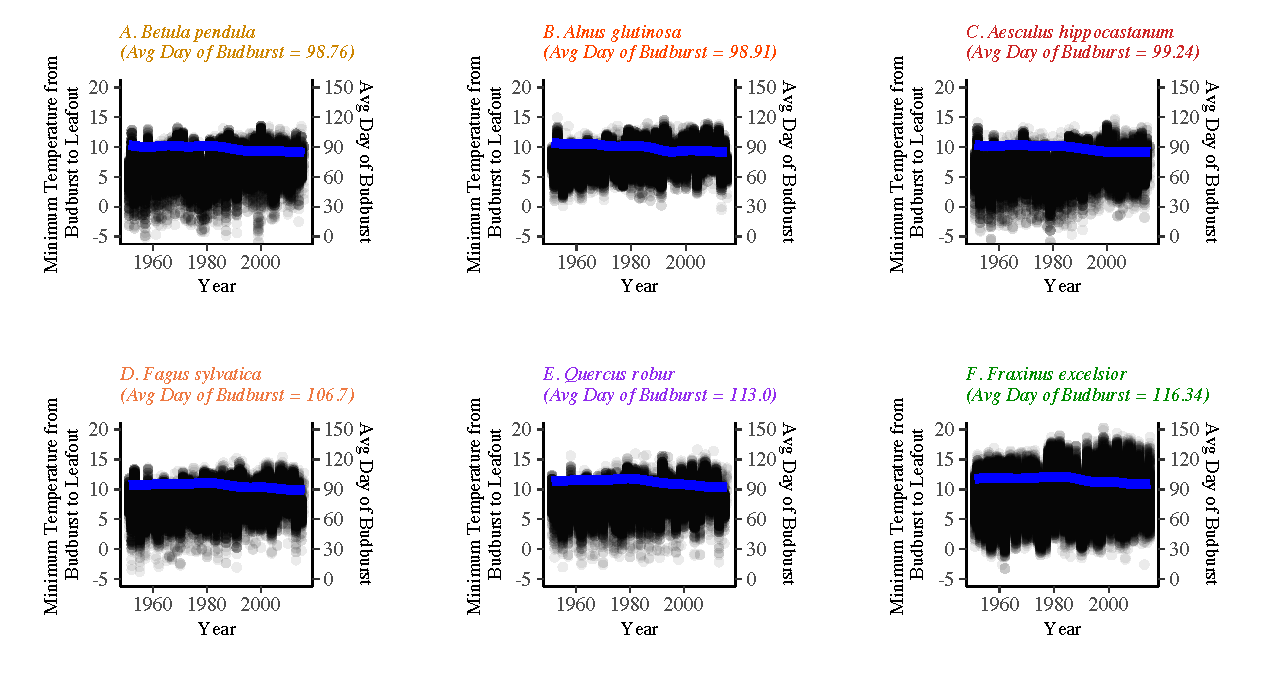
\includegraphics[width=16cm]{..//analyses/figures/MSTBB_bySpp.png}
  -\caption{Mean spring temperatures are plotted for each site and year (from 1951-2016) for each species. The blue line is a smoothing spline, indicating the trend of average day of budburst for each year for each species. Species are ordered by average day of budburst, with the earliest being \textit{Betula pendula} and the latest being \textit{Fraxinus excelsior} and species names are color-coded to match the other figures. }\label{fig:mst}
  -\end{center}
  -\end{figure}}

\iffalse
\begin{equation} \label{eq:3}
lm(\text{Minimum Temperature \degree{C}} $\sim$ \text{Climate Change} (scaled))
\end{equation}
\fi

% latex table generated in R 3.6.0 by xtable 1.8-4 package
% Thu Sep 19 17:09:41 2019
\begin{table}[H]
\centering
\caption{Summary of simple linear regression model of day of budburst before and after climate change.} 
\begin{tabular}{lrrr}
  \hline
 & Estimate & 10\% & 90\% \\ 
  \hline
Intercept & 104.88 & 104.85 & 104.90 \\ 
  Climate Change & -5.88 & -5.93 & -5.83 \\ 
   \hline
\end{tabular}
\end{table}
% latex table generated in R 3.6.0 by xtable 1.8-4 package
% Thu Sep 19 17:09:41 2019
\begin{table}[H]
\centering
\caption{Summary of simple linear regression model of day of year of last freeze (-2.2°C) before and after climate change.} 
\begin{tabular}{lrrr}
  \hline
 & Estimate & 10\% & 90\% \\ 
  \hline
Intercept & 128.87 & 128.84 & 128.89 \\ 
  Climate Change & -5.86 & -5.92 & -5.81 \\ 
   \hline
\end{tabular}
\end{table}
% latex table generated in R 3.6.0 by xtable 1.8-4 package
% Thu Sep 19 17:09:42 2019
\begin{table}[H]
\centering
\caption{Summary of simple linear regression model of average minimum temperature between budburst and leafout before and after climate change.} 
\begin{tabular}{lrrr}
  \hline
 & Estimate & 10\% & 90\% \\ 
  \hline
Intercept & 7.17 & 7.16 & 7.17 \\ 
  Climate Change & 0.81 & 0.80 & 0.82 \\ 
   \hline
\end{tabular}
\end{table}



\begin{kframe}


{\ttfamily\noindent\bfseries\color{errorcolor}{\#\# Error in `[.data.frame`(x, r, vars, drop = drop): undefined columns selected}}\end{kframe}% latex table generated in R 3.6.0 by xtable 1.8-4 package
% Thu Sep 19 17:09:42 2019
\begin{table}[H]
\centering
\caption{Summary of main Bernouilli model of false spring risk without the species interactions (estimates presented on logit scale for \textit{Aesculus hippocastanum}).} 
\begin{tabular}{lrrrrr}
  \hline
 & Estimate & 10\% & 90\% & Species & NA \\ 
  \hline
Aesculus hippocastanum & 0.12 & 0.16 & 0.14 & 7.80 & NAO Index \\ 
  Aesculus hippocastanum & -0.50 & -0.45 & -0.48 & 10.80 & Mean Spring 
Temperature \\ 
  Aesculus hippocastanum & 0.38 & 0.43 & 0.40 & 9.80 & Distance from 
Coast \\ 
  Aesculus hippocastanum & 0.16 & 0.22 & 0.19 & 8.80 & Elevation \\ 
  Aesculus hippocastanum & -0.08 & -0.05 & -0.06 & 6.80 & Space Parameter \\ 
  Aesculus hippocastanum & 0.33 & 0.37 & 0.35 & 5.80 & Climate Change \\ 
  Alnus glutinosa & 0.01 & 0.13 & 0.07 & 7.75 & NAO Index \\ 
  Betula pendula & 0.01 & 0.11 & 0.06 & 7.70 & NAO Index \\ 
  Fagus sylvatica & 0.21 & 0.32 & 0.26 & 7.65 & NAO Index \\ 
  Fraxinus excelsior & 0.10 & 0.24 & 0.17 & 7.60 & NAO Index \\ 
  Quercus robur & 0.16 & 0.28 & 0.22 & 7.55 & NAO Index \\ 
  Alnus glutinosa & -0.40 & -0.27 & -0.33 & 10.75 & Mean Spring 
Temperature \\ 
  Betula pendula & -0.55 & -0.44 & -0.50 & 10.70 & Mean Spring 
Temperature \\ 
  Fagus sylvatica & -0.60 & -0.48 & -0.54 & 10.65 & Mean Spring 
Temperature \\ 
  Fraxinus excelsior & -0.24 & -0.07 & -0.16 & 10.60 & Mean Spring 
Temperature \\ 
  Quercus robur & -0.44 & -0.31 & -0.37 & 10.55 & Mean Spring 
Temperature \\ 
  Alnus glutinosa & 0.27 & 0.40 & 0.33 & 9.75 & Distance from 
Coast \\ 
  Betula pendula & 0.35 & 0.47 & 0.41 & 9.70 & Distance from 
Coast \\ 
  Fagus sylvatica & 0.34 & 0.46 & 0.40 & 9.65 & Distance from 
Coast \\ 
  Fraxinus excelsior & 0.58 & 0.74 & 0.66 & 9.60 & Distance from 
Coast \\ 
  Quercus robur & 0.23 & 0.37 & 0.30 & 9.55 & Distance from 
Coast \\ 
  Alnus glutinosa & 0.14 & 0.29 & 0.21 & 8.75 & Elevation \\ 
  Betula pendula & 0.16 & 0.29 & 0.22 & 8.70 & Elevation \\ 
  Fagus sylvatica & 0.12 & 0.26 & 0.19 & 8.65 & Elevation \\ 
  Fraxinus excelsior & -0.27 & -0.09 & -0.18 & 8.60 & Elevation \\ 
  Quercus robur & 0.03 & 0.19 & 0.11 & 8.55 & Elevation \\ 
  Alnus glutinosa & -0.10 & 0.00 & -0.05 & 6.75 & Space Parameter \\ 
  Betula pendula & -0.12 & -0.03 & -0.07 & 6.70 & Space Parameter \\ 
  Fagus sylvatica & -0.16 & -0.06 & -0.11 & 6.65 & Space Parameter \\ 
  Fraxinus excelsior & -0.08 & 0.05 & -0.01 & 6.60 & Space Parameter \\ 
  Quercus robur & -0.10 & 0.01 & -0.05 & 6.55 & Space Parameter \\ 
  Alnus glutinosa & 0.36 & 0.47 & 0.41 & 5.75 & Climate Change \\ 
  Betula pendula & 0.36 & 0.46 & 0.41 & 5.70 & Climate Change \\ 
  Fagus sylvatica & -0.02 & 0.08 & 0.03 & 5.65 & Climate Change \\ 
  Fraxinus excelsior & -0.23 & -0.10 & -0.17 & 5.60 & Climate Change \\ 
  Quercus robur & -0.11 & 0.00 & -0.05 & 5.55 & Climate Change \\ 
  Overall Estimate & 0.10 & 0.21 & 0.15 & 8.00 & NAO Index \\ 
  Overall Estimate & -0.45 & -0.34 & -0.40 & 11.00 & Mean Spring 
Temperature \\ 
  Overall Estimate & 0.36 & 0.48 & 0.42 & 10.00 & Distance from 
Coast \\ 
  Overall Estimate & 0.06 & 0.19 & 0.13 & 9.00 & Elevation \\ 
  Overall Estimate & -0.11 & -0.01 & -0.06 & 7.00 & Space Parameter \\ 
  Overall Estimate & 0.11 & 0.21 & 0.16 & 6.00 & Climate Change \\ 
  Overall Estimate & -0.85 & -0.81 & -0.83 & 2.00 & NAO Index:Climate Change \\ 
  Overall Estimate & 0.40 & 0.44 & 0.42 & 5.00 & Mean Spring 
Temperature:Climate Change \\ 
  Overall Estimate & -0.15 & -0.10 & -0.12 & 4.00 & Distance from 
Coast:Climate Change \\ 
  Overall Estimate & -0.03 & 0.03 & -0.00 & 3.00 & Elevation:Climate Change \\ 
  Overall Estimate & -0.07 & -0.03 & -0.05 & 1.00 & Space Parameter:Climate Change \\ 
   \hline
\end{tabular}
\end{table}



\iffalse
{\begin{figure} [H]
\begin{subfigure}{.5\textwidth}
  \centering
  \includegraphics[width=6cm]{..//analyses/figures/PPCs/orig_ppc.png}
  \caption{}
  \label{fig:sfig1}
\end{subfigure}%
\begin{subfigure}{.5\textwidth}
  \centering
  \includegraphics[width=6cm]{..//analyses/figures/PPCs/ppc_sd.png}
  \caption{}
  \label{fig:sfig2}
\end{subfigure}
\caption{(a) Posterior predictive check comparing the simulated model estimates to the raw data. The curves overlap greatly, which suggests our model is valid and fit the data. (b) Posterior predictive check comparing the standard deviation from our model output to the data. The model fits our data well, which suggests our model is valid.} %IMC: the fit between data and predictions is pretty tight so I'm aware that perhaps this is not necessary, but as a reviewer I would like to see some quantification of that model accuracy (pseudo-R² is an alternative, but any other could work too). 
\label{fig:suppppc}
\end{figure}}
\fi

{\begin{figure} [H]
  -\begin{center}
  -\includegraphics[width=16cm]{..//analyses/figures/APC_allpred_allspp_baseR.pdf}
  -\caption{Average predictive comparisons for all climate change interactions with each of the main effects (i.e., mean spring temperature, distance from the coast, elevation, and NAO index) for all species. }\label{fig:suppapc}
  -\end{center}
  -\end{figure}}
  
  {\begin{figure} [H]
  -\begin{center}
  -\includegraphics[width=12cm]{..//analyses/figures/model_output_90_dvr.png}
  -\caption{Model output with different durations of vegetative risk for each species. More positive values indicate an increased probability of a false spring whereas more negative values suggest a lower probability of a false spring. Dots and lines show means and 10\% uncertainty intervals. Values closer to zero have less of an effect on false springs. There were 622,565 zeros and 132,463 ones for false springs in the data.}\label{fig:dvr}
  -\end{center}
  -\end{figure}}
  
% latex table generated in R 3.6.0 by xtable 1.8-4 package
% Thu Sep 19 17:09:42 2019
\begin{table}[H]
\centering
\caption{Summary of Bernouilli model of false spring risk with varying durations of vegetative risk for each species without the species interactions (estimates presented on logit scale for \textit{Aesculus hippocastanum}).} 
\begin{tabular}{lrrrrr}
  \hline
 & Estimate & 10\% & 25\% & 75\% & 90\% \\ 
  \hline
NAO Index & 0.15 & 0.13 & 0.14 & 0.16 & 0.17 \\ 
  Mean Spring 
Temperature & -0.50 & -0.53 & -0.51 & -0.49 & -0.48 \\ 
  Distance from 
Coast & 0.40 & 0.38 & 0.39 & 0.42 & 0.43 \\ 
  Elevation & 0.15 & 0.12 & 0.14 & 0.16 & 0.18 \\ 
  Space Parameter & -0.06 & -0.08 & -0.07 & -0.06 & -0.04 \\ 
  Climate Change & 0.34 & 0.32 & 0.34 & 0.35 & 0.37 \\ 
  NAO Index by Climate Change & -0.64 & -0.68 & -0.65 & -0.62 & -0.59 \\ 
  Mean Spring 
Temperature by Climate Change & 0.59 & 0.54 & 0.57 & 0.61 & 0.64 \\ 
  Distance from 
Coast by Climate Change & -0.17 & -0.22 & -0.19 & -0.14 & -0.11 \\ 
  Elevation by Climate Change & 0.13 & 0.08 & 0.11 & 0.15 & 0.19 \\ 
  Space Parameter by Climate Change & -0.07 & -0.11 & -0.09 & -0.06 & -0.04 \\ 
   \hline
\end{tabular}
\end{table}


{\begin{figure} [H]
  -\begin{center}
  -\includegraphics[width=12cm]{..//analyses/figures/model_output_90_five.png}
  -\caption{Model output with a lower temperature threshold (-5$^{\circ}$C) for defining a false spring. More positive values indicate an increased probability of a false spring whereas more negative values suggest a lower probability of a false spring. Dots and lines show means and 10\% uncertainty intervals. Values closer to zero have less of an effect on false springs. There were 730,996 zeros and 23,855 ones for false springs in the data.}\label{fig:five}
  -\end{center}
  -\end{figure}}
  
% latex table generated in R 3.6.0 by xtable 1.8-4 package
% Thu Sep 19 17:09:42 2019
\begin{table}[H]
\centering
\caption{Summary of Bernouilli model of false spring risk with a lower temperature threshold (-5$^{\circ}$C) for defining a false spring without the species interactions (estimates presented on logit scale for \textit{Aesculus hippocastanum}).} 
\begin{tabular}{lrrrrr}
  \hline
 & Estimate & 10\% & 25\% & 75\% & 90\% \\ 
  \hline
NAO Index & 0.09 & 0.05 & 0.07 & 0.11 & 0.14 \\ 
  Mean Spring 
Temperature & -0.72 & -0.77 & -0.74 & -0.70 & -0.67 \\ 
  Distance from 
Coast & 0.21 & 0.15 & 0.18 & 0.23 & 0.27 \\ 
  Elevation & 0.63 & 0.58 & 0.61 & 0.65 & 0.68 \\ 
  Space Parameter & -0.02 & -0.06 & -0.04 & 0.00 & 0.03 \\ 
  Climate Change & 0.58 & 0.53 & 0.56 & 0.60 & 0.63 \\ 
  NAO Index by Climate Change & -0.92 & -1.02 & -0.96 & -0.88 & -0.83 \\ 
  Mean Spring 
Temperature by Climate Change & 0.64 & 0.55 & 0.60 & 0.69 & 0.74 \\ 
  Distance from 
Coast by Climate Change & 0.01 & -0.10 & -0.03 & 0.06 & 0.13 \\ 
  Elevation by Climate Change & -0.24 & -0.35 & -0.29 & -0.20 & -0.14 \\ 
  Space Parameter by Climate Change & -0.04 & -0.13 & -0.08 & -0.01 & 0.05 \\ 
   \hline
\end{tabular}
\end{table}

  

%{\begin{figure} [H]
%  -\begin{center}
%  -\includegraphics[width=16cm]{..//figures/PropSitesbyYrwBB.png}
%  -\caption{The black line indicates the proportion of sites that had false spring conditions for each year across all species. The blue line is a smoothing spline, indicating the trend of average day of budburst for each year for each species. Species are ordered by average day of budburst, with the earliest being \textit{Betula pendula} and the latest being \textit{Fraxinus excelsior}.}\label{fig:fsprop}
%  -\end{center}
%  -\end{figure}}

\end{document}
